\documentclass{article}
\usepackage[utf8]{inputenc}
\usepackage{geometry}
\usepackage{enumitem}
\usepackage{hyperref}
\usepackage{xcolor}
\usepackage{graphicx}
\usepackage{array}
\usepackage{multirow}
\usepackage{amsmath, amssymb}
\usepackage{chemfig}
\usepackage{mhchem}
\usepackage{tikz}
\usepackage{setspace}
\usepackage{soul}
\usepackage{mathtools}
\usepackage{booktabs}
\usepackage{chemformula}
\usepackage{siunitx}
\usetikzlibrary{positioning, shapes, arrows.meta, decorations.pathreplacing, fit, backgrounds}
\usepackage{longtable}
\geometry{margin=1in}
\setlength{\parskip}{0.5em}

\begin{document}

\begin{center}
    {\LARGE \textbf{SI Session Planning Form}}
\end{center}

\vspace{0.5cm}

\noindent
\begin{flushleft}
\textbf{SI Leader:} Brandon Cobb \\
\textbf{Session Week:} 1 \\
\textbf{Session \#:} 1 \\
\textbf{Instructor:} Professor Tramontozzi \\
\textbf{Old Plans:} \href{https://macombedu.sharepoint.com/:b:/s/ASC-SupplementalInstructionEmbeddedTutoring/EeSYqCwT_KhMolgJvXbVEjgBOyF_DevvS8BgCm1zPkQQJg?e=QJTt4o}{SharePoint} \\
\textbf{Session Goal:} Students will be able to calculate the missing numerical value for subscripts on elements in incomplete molecules, knowing its formula unit number, and define matter, its phases and both chemical and physical properties of it.
\end{flushleft}

\vspace{1em}
\section*{\underline{Opener}}
{\centering\large\textbf{\hl{Take Attendance}}\par}\vspace{-0.25\baselineskip}

\\
\begin{tabular}{|p{4.2cm}|p{9.8cm}|}
\hline
\textbf{Collaborative Learning Techniques} & Clusters \\
\hline
\textbf{Learning Strategy} & Think Aloud \\
\hline
\textbf{Time} & 12:00---12:10 \\
\hline
\textbf{Materials} & A number of periodic tables with group numbers on them, pen, paper, ready to speak \\
\hline
\textbf{Lecture/Textbook/Old Plans/Slide References} & ptable.com, class roster, Chapter 1: Basic Concepts About Matter \\
\hline
\end{tabular}

\vspace{0.5cm}
\noindent
{\large \textbf{Instructions (please provide a \hl{DETAILED} activity breakdown below (and/or attached}} \\

\begin{tabular}{|p{0.9\linewidth}|}
\hline

\vspace{0.2cm}
1. The leader will arrange group posters into far apart places in the classroom. \\
2. Each group will be informated of how many group members decided to be in which groups. \\
3. Each group will be given a riddle. \\[0.5em]
\begin{centering}
    \emph{Split me clean and I become the table itself.} \\
    \emph{Who of us can be fully written in stones of fire and metal?} \\
\end{centering}
\\[0.5em]
1. As a group, learn eachother's names, and their spelling (write the first names out). We will organize seating into a circle with pen and paper. \\
2. Take a minute to pick your own solution to the riddle. \\
3. If you can't, when the group reconvenes after 2 minutes, state you have no answer to the group, otherwise write your solution down. \\
4. Point out the Leader is part of every group (BRaNdON). \\[0.5em]
1. In 2 minutes, the groups will be asked to reconvene and pick a group answer. I'll check if the groups have any idea. If not, I'll give them a hint about my name being an answer. \\
2. We'll talk about how first chosing clusters by our own volition, or forced creates groups of effectively different sizes and can change the variety of answers offered. \\
3. I'll share the research piece \href{https://pubs.acs.org/doi/pdf/10.1021/ed077p111?ref=article_openPDF}{Student Perspectives on Small-Group Learning in Chemistry} and we'll transition into the first activity
\hline
\end{tabular}
\newpage

\noindent
{\large \textbf{Content (fully worked out problems \& answers)}} \\[0.2em]
\noindent
\begin{tabular}{|p{0.9\linewidth}|}
\hline
\vspace{0.2cm}
\textbf{(1)}. Define matter in your own words. List two essential characteristics that distinguish matter from forms of energy. \\
\hline
\textbf{Solution:} Matter is anything that has mass and occupies space. Two key characteristics are: \\ 
\begin{enumerate}
    \item it has measurable mass
    \item it takes up volume
\end{enumerate}
\\
\hline
\end{tabular}
\newpage
\begin{tabular}{|p{0.9\linewidth}|}
\hline
\vspace{0.2cm}

\textbf{(2)} Classify each of the following as a pure substance or a mixture: \\
\begin{enumerate}
    \item sodium chloride
    \item air
    \item copper
    \item seawater 
\end{enumerate}\\
\hline
\textbf{Solution:} \\
\begin{enumerate}
    \item pure substance
    \item mixture
    \item pure substance
    \item mixture
\end{enumerate}
\\
\hline
\end{tabular}
\newpage
\begin{tabular}{|p{0.9\linewidth}|}
\hline

\vspace{0.2cm}

\textbf{(3)} Explain the difference between an element and a compound. Give one example of each. \\
\hline

\textbf{Solution:} \\
An element is a substance made of only one type of atom (e.g., oxygen). A compound contains two or more elements chemically bonded together (e.g., water). \\
\hline
\end{tabular}
\newpage
\\
\begin{tabular}{|p{0.9\linewidth}|}
\hline
\vspace{0.2cm}

\textbf{(4)} State whether each of the following is a physical property or a chemical property: \\
\begin{enumerate}
    \item melting point of ice
    \item flammability of hydrogen gas
    \item density of aluminum
    \item ability of iron to rust
\end{enumerate}
\hline

\textbf{Solution:} \\
\begin{enumerate}
    \item physical
    \item chemical
    \item physical
    \item chemical 
\end{enumerate}
\\
\hline
\end{tabular}
\newpage
\begin{tabular}{|p{0.9\linewidth}|}
\hline
\vspace{0.2cm}

\textbf{(5)} Identify whether the following changes are physical or chemical: \\
\begin{enumerate}
    \item evaporation of alcohol
    \item burning of a candle
    \item dissolving sugar in water
    \item digestion of food
\end{enumerate} \\
\hline
\textbf{Solution:} \\
\begin{enumerate}
    \item physical
    \item chemical
    \item physical
    \item chemical
\end{enumerate}
\\
\hline
\end{tabular}
\newpage
\noindent
{\large \textbf{Content (fully worked out problems \& answers)}} \\[0.2em]
\noindent
\begin{tabular}{|p{0.9\linewidth}|}
\hline
\vspace{0.2cm}

\textbf{(6)} Name the three classical states of matter. For each state, describe the arrangement and motion of particles. \\
\hline
\textbf{Solution:} Solids have particles closely packed in fixed positions with only vibrations. Liquids have particles close but able to slide past each other. Gases have particles far apart, moving freely at high speeds. \\
\hline
\end{tabular}
\newpage
\begin{tabular}{|p{0.9\linewidth}|}
\hline
\vspace{0.2cm}

\textbf{(7)} Distinguish between intensive and extensive properties. Classify the following as intensive or extensive: \\
\begin{enumerate}
    \item mass
    \item color
    \item volume
    \item boiling point
\end{enumerate}
\\
\hline
\textbf{Solution:} \\
Intensive properties do not depend on amount, while extensive properties do. \\
\begin{enumerate}
    \item extensive
    \item intensive
    \item extensive
    \item intensive
\end{enumerate}
\\
\hline
\end{tabular}
\newpage
\begin{tabular}{|p{0.9\linewidth}|}
\hline
\vspace{0.2cm}

\textbf{(8)} State the law of conservation of mass. Why is this law important in chemical reactions? \\
\hline
\textbf{Solution:} \\
The law states that mass is neither created nor destroyed in a chemical reaction. It ensures that the mass of products equals the mass of reactants, allowing balanced equations and stoichiometry. \\
\hline
\end{tabular}
\newpage
\begin{tabular}{|p{0.9\linewidth}|}
\hline
\vspace{0.2cm}

\textbf{(9)} Briefly state Dalton’s main postulates of the atomic theory. Which of these postulates are no longer considered correct? \\
Postulates:
\begin{enumerate} 
    \item all matter is made of indivisible atoms
    \item atoms of the same element are identical
    \item atoms combine in whole-number ratios
    \item atoms rearrange in reactions but are not created or destroyed. 
\end{enumerate}
\hline
\textbf{Solution:} \\
    \item Today, (1) is not correct (atoms are divisible into subatomic particles), and (2) is not fully correct (isotopes exist). \\
\hline
\end{tabular}
\newpage
\begin{tabular}{|p{0.9\linewidth}|}
\hline
\vspace{0.2cm}

\textbf{(10)} Draw a simple classification chart of matter showing how substances divide into pure substances and mixtures, and how they divide (respectively). \\
\hline
\textbf{Solution:} \\
Matter can be divided into: \\
\quad Pure Substances $\rightarrow$ Elements vs. Compounds \\
\quad Mixtures $\rightarrow$ Homogeneous (uniform, e.g., air) vs. Heterogeneous (non-uniform, e.g., salad). \\
\hline
\end{tabular}
\newpage
\noindent
{\large \textbf{Checking for Understanding (questions \& answers)}} \\

\begin{tabular}{|p{0.9\linewidth}|}
\hline
\textbf{(1)} Is light considered matter? Why or why not? \\ 
\textbf{Solution:} No — light is electromagnetic radiation, not matter. Light is carried by photons (symbol $\gamma$), which have zero rest mass ($m_0 = 0$) yet carry energy ($E = h\nu$) and momentum ($p = h/\lambda$). Matter, by the usual definition, consists of particles that have rest mass and occupy space; photons do not, so they are classified as energy. \\ \hline
\end{tabular}
\newpage
\begin{tabular}{|p{0.9\linewidth}|}
\hline
\textbf{(2)} If you filter seawater, what happens to its classification as a mixture? \\ 
\textbf{Solution:} Filtration removes heterogeneous suspended solids, but dissolved ions remain. Dissolved species such as $Na^+$ and $Cl^-$ remain uniformly distributed. Therefore, seawater remains a homogeneous mixture (solution) after filtration. \\ \hline
\end{tabular}
\newpage
\begin{tabular}{|p{0.9\linewidth}|}
\hline
\textbf{(3)} Why is water (H$_2$O) a compound and not an element? \\ 
\textbf{Solution:} Water contains two different elements (hydrogen and oxygen) in a fixed ratio. An element consists of only one type of atom; a compound consists of two or more types chemically bonded. Breaking water into $H_2$ and $O_2$ requires a chemical reaction: $$2\,H_2O \rightarrow 2\,H_2 + O_2.$$ \\ \hline
\end{tabular}
\newpage
\begin{tabular}{|p{0.9\linewidth}|}
\hline
\textbf{(4)} When salt dissolves in water, why is this considered a physical change? \\
\textbf{Solution:} Salt dissociates into ions: $$NaCl_{(s)} \rightarrow Na^+_{(aq)} + Cl^-_{(aq)}.$$ No new chemical species are formed; chemical identity of ions remains. The process is reversible (e.g., evaporation reforms $NaCl_{(s)}$). \\ \hline
\end{tabular}
\newpage
\begin{tabular}{|p{0.9\linewidth}|}
\hline
\textbf{(5)} Which state of matter has a definite shape and a definite volume? \\
\textbf{Solution:} Solids have definite shape and definite volume. Liquids have definite volume but indefinite shape. Gases have neither definite shape nor definite volume. \\ \hline
\end{tabular}
\newpage
\begin{tabular}{|p{0.9\linewidth}|}
\hline
\textbf{(6)} Why must the total mass of reactants equal the total mass of products in a closed system? \\
\textbf{Solution:} Atoms are rearranged but not created or destroyed. Total mass is conserved: $$\sum m_{\text{reactants}} = \sum m_{\text{products}}.$$ Example: $$2\,H_2 + O_2 \rightarrow 2\,H_2O$$ rearranges the same atoms; mass is unchanged. \\ \hline
\end{tabular}
\newpage
\begin{tabular}{|p{0.9\linewidth}|}
\hline
\textbf{(7)} Give an everyday example of a homogeneous mixture and a heterogeneous mixture. \\
\textbf{Solution:} Homogeneous mixture: $NaCl_{(aq)}$, air — composition is uniform. Heterogeneous mixture: salad, sand + water — composition varies visibly. \\ \hline
\end{tabular}
\newpage
\noindent
\section*{\underline{Activity 1}}
\begin{tabular}{|p{4.2cm}|p{9.8cm}|}
\hline
\textbf{Collaborative Learning Techniques} & Think---Pair---Share \\
\hline
\textbf{Learning Strategy} & Think Aloud \\
\hline
\textbf{Time} & 12:10---12:50 \\
\hline
\textbf{Materials} & Computers, draw.io, usb-c to hdmi, projector \\
\hline
\textbf{Lecture/Textbook/Old Plans/Slide References} & Chapter 1: Basic Concepts of Matter \\
\hline
\end{tabular}

\vspace{0.5cm}

\noindent
{\large \textbf{Instructions (please provide a \hl{DETAILED} activity breakdown below (and/or attached}} \\


\begin{tabular}{|p{0.9\linewidth}|}
\hline
\begin{enumerate}
    \item \textbf{Think---Pair---Share:} Group members work on an assignment or project individually and then share their results with a partner. After discussing with a partner, share findings with the larger group.
    \item \textbf{Activity 1}
    \item \textbf{Objective:} Students will explore a preloaded \texttt{draw.io} diagram containing terms and images. They will practice organizing information, creating shapes, and collaboratively constructing knowledge through the Think--Pair--Share method.
    \begin{enumerate}
        \item \textbf{Prepare the Resource:}
        \begin{itemize}
            \item Upload the \texttt{.drawio} file to a hosting service and ensure that each student will access a personal copy.
            \item Place the activity link on the course website under \emph{Chapter One Resources} titled \textbf{Drawio.com Activity}.
            \item Test the link to confirm that it opens a fresh drawing board instance for every student.
        \end{itemize}
    
        \item \textbf{Student Access:}
        \begin{itemize}
            \item Students click the link from the course website.
            \item Each student is taken to their own copy of the drawing environment with preloaded definitions, terms, and images.
        \end{itemize}
    
        \item \textbf{Think--Pair--Share Structure:}
        \begin{enumerate}
            \item \textbf{Think:} Students work individually in their drawing board, experimenting with organizing terms, definitions, and adding at least one custom shape.
            \item \textbf{Pair:} Each student discusses their organization and choices with a partner, comparing and contrasting their diagrams.
            \item \textbf{Share:} Pairs then present their key findings and reasoning to the larger group.
        \end{enumerate}
    
        \item \textbf{Instructor Orchestration:}
        \begin{itemize}
            \item As pairs share their reasoning, integrate their decisions into the \emph{master notebook} displayed on the board.
            \item Encourage students to justify their organizational choices and connections between terms.
            \item Highlight strong examples of creativity or clarity in structuring the diagrams.
        \end{itemize}
    
        \item \textbf{Learning Outcome:}
        \begin{itemize}
            \item Students gain familiarity with diagramming tools and collaborative knowledge-building.
            \item They learn to independently structure information and then negotiate meaning with peers.
        \end{itemize}
    \end{enumerate}\\
\hline
\end{tabular}
\newpage
\begin{tabular}{|p{0.9\linewidth}|}
\hline
\textbf{Example Diagram of Shape Connections:}

\begin{center}
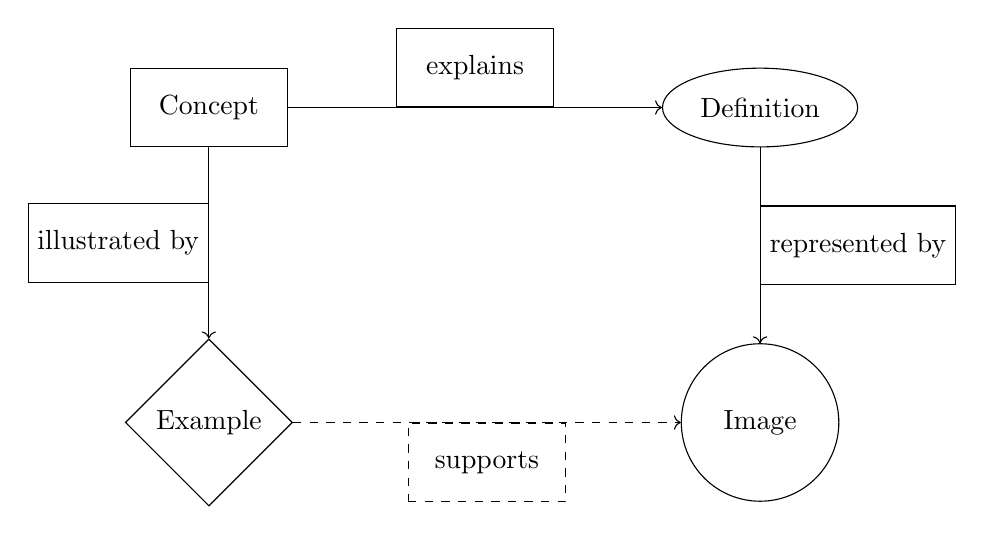
\begin{tikzpicture}[node distance=2cm, every node/.style={draw, minimum width=2cm, minimum height=1cm}]
    \node (concept) [rectangle] {Concept};
    \node (definition) [ellipse, right of=concept, xshift=5cm] {Definition};
    \node (example) [diamond, below of=concept, yshift=-2cm] {Example};
    \node (image) [circle, below of=definition, yshift=-2cm] {Image};

    \draw[->] (concept) -- (definition) node[midway, above] {explains};
    \draw[->] (concept) -- (example) node[midway, left] {illustrated by};
    \draw[->] (definition) -- (image) node[midway, right] {represented by};
    \draw[->, dashed] (example) -- (image) node[midway, below] {supports};
\end{tikzpicture}
\end{center}

\\ \hline
\end{tabular}
\newpage

\noindent
\noindent
{\large \textbf{Content (fully worked out problems \& answers)}} \\

% Question 1: Parallel Process Branches
\begin{longtable}{|p{0.9\linewidth}|}
\hline
\textbf{(1)} How do you create parallel process branches that split from a single node, similar to draw.io’s forked flow? \\[0.5em]
\textbf{Solution:} \\[0.5em]
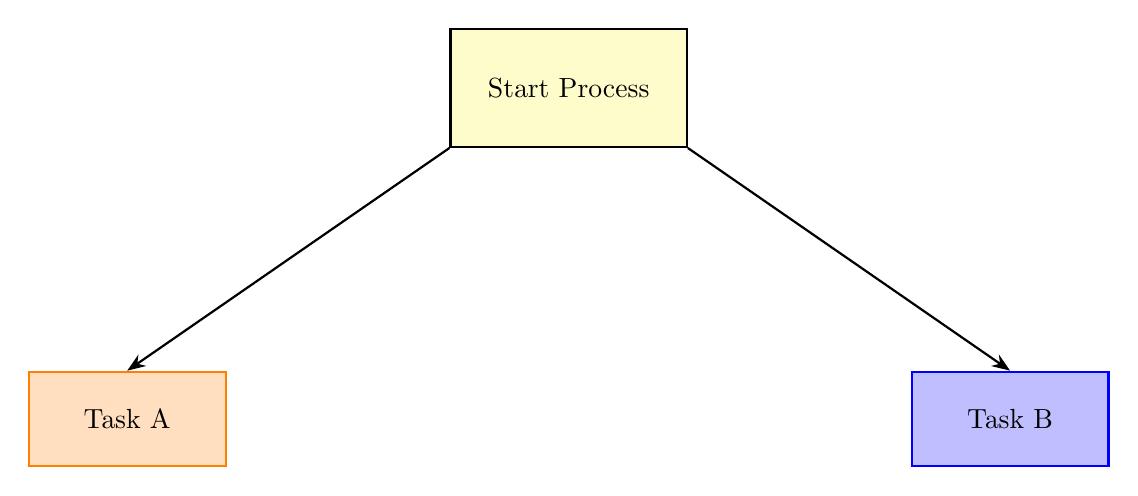
\begin{tikzpicture}[baseline=(current bounding box.center), node distance=4cm]
\node[
    draw=black,
    thick,
    rectangle,
    minimum width=3cm,
    minimum height=1.5cm,
    align=center,
    fill=yellow!20
] (start) {Start Process};
\node[
    draw=orange,
    thick,
    rectangle,
    minimum width=2.5cm,
    minimum height=1.2cm,
    align=center,
    fill=orange!25,
    below left=of start
] (branchA) {Task A};
\node[
    draw=blue,
    thick,
    rectangle,
    minimum width=2.5cm,
    minimum height=1.2cm,
    align=center,
    fill=blue!25,
    below right=of start
] (branchB) {Task B};
\draw[-Stealth, thick, black] (start.south west) -- (branchA.north);
\draw[-Stealth, thick, black] (start.south east) -- (branchB.north);
\end{tikzpicture} \\[0.5em]
\textbf{Draw.io Translation:} Create a single rectangle for start. Add two rectangles below and connect using straight or elbow connectors to show branching. \\[0.5em]
\textbf{Key Parameters:} Node positions \texttt{below left} and \texttt{below right}, straight arrow style \texttt{-Stealth, thick} \\
\hline
\end{longtable}

\newpage
\noindent
{\large \textbf{Content (fully worked out problems \& answers)}} \\

% Question 1: Annotated Notes/Comments
\begin{longtable}{|p{0.9\linewidth}|}
\hline
\textbf{(2)} How do you add annotation notes or comments near a process node, like draw.io’s sticky notes or text labels? \\[0.5em]
\textbf{Solution:} \\[0.5em]
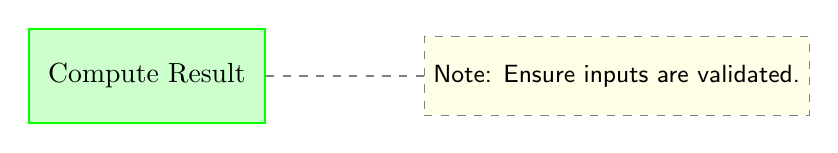
\begin{tikzpicture}[baseline=(current bounding box.center)]
\node[
    draw=green,
    thick,
    rectangle,
    minimum width=3cm,
    minimum height=1.2cm,
    align=center,
    fill=green!20
] (process) {Compute Result};
\node[
    draw=gray,
    dashed,
    rectangle,
    minimum width=2.5cm,
    minimum height=1cm,
    align=left,
    fill=yellow!10,
    font=\sffamily\small,
    right=of process,
    xshift=1cm
] (note) {Note: Ensure inputs are validated.};
\draw[dashed, thin, gray, -] (process.east) -- (note.west);
\end{tikzpicture} \\[0.5em]
\textbf{Draw.io Translation:} Use Rectangle or Sticky Note shape for annotation. Connect with dashed line. Set fill color light yellow, dashed connector. \\[0.5em]
\textbf{Key Parameters:} \texttt{dashed, thin, gray} for lines, \texttt{fill=yellow!10} for note background \\
\hline
\end{longtable}

\newpage
\noindent
{\large \textbf{Content (fully worked out problems \& answers)}} \\

% Question 13: Swimlane Diagram Section
\begin{longtable}{|p{0.9\linewidth}|}
\hline
\textbf{(3)} How do you create swimlane sections for departments or roles, matching draw.io swimlane shapes? \\[0.5em]
\textbf{Solution:} \\[0.5em]
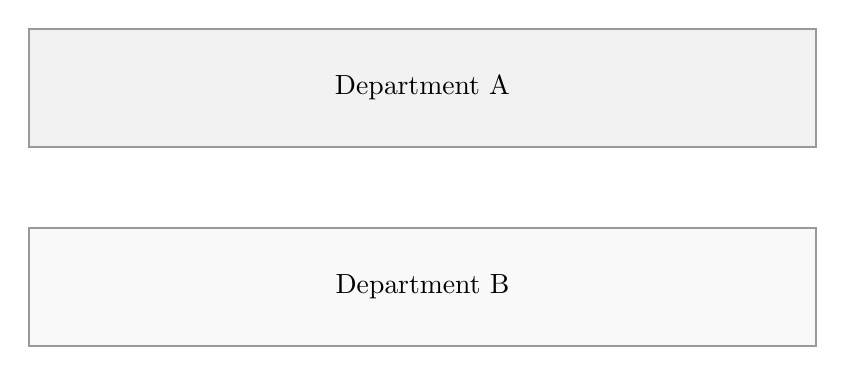
\begin{tikzpicture}[baseline=(current bounding box.center)]
\node[
    draw=gray!80,
    thick,
    rectangle,
    minimum width=10cm,
    minimum height=1.5cm,
    align=center,
    fill=gray!10
] (lane1) {Department A};
\node[
    draw=gray!80,
    thick,
    rectangle,
    minimum width=10cm,
    minimum height=1.5cm,
    align=center,
    fill=gray!05,
    below=of lane1
] (lane2) {Department B};
\end{tikzpicture} \\[0.5em]
\textbf{Draw.io Translation:} Use horizontal or vertical swimlane shape. Set width=full page, assign alternating fill colors per lane. \\[0.5em]
\textbf{Key Parameters:} \texttt{rectangle, minimum width=10cm, minimum height=1.5cm, fill=gray!10/gray!05} \\
\hline
\end{longtable}
\newpage
\noindent
{\large \textbf{Content (fully worked out problems \& answers)}} \\

% Question 14: Multi-decision Flow
\begin{longtable}{|p{0.9\linewidth}|}
\hline
\textbf{(4)} How do you create multiple consecutive decision nodes with branching paths, similar to complex draw.io decision flows? \\[0.5em]
\textbf{Solution:} \\[0.5em]
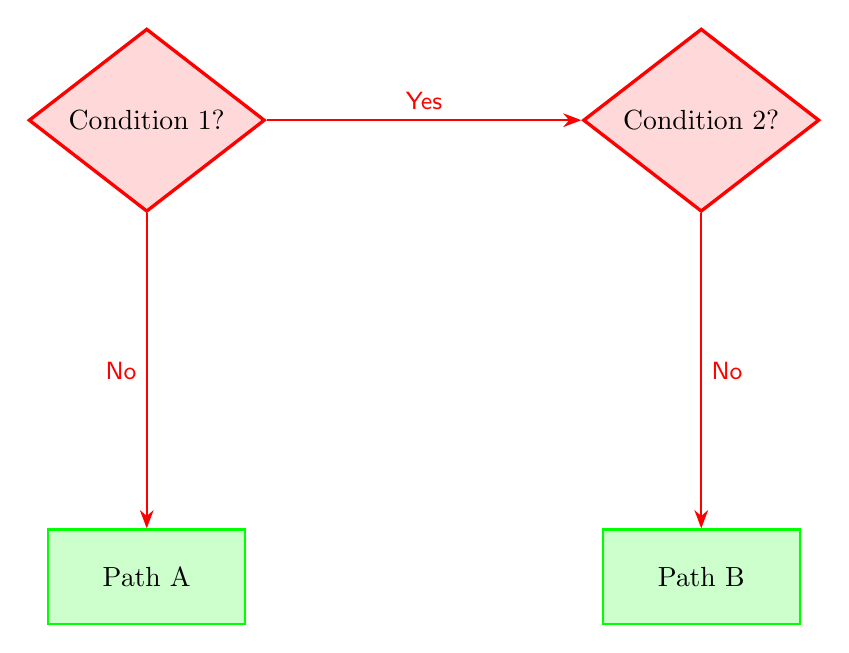
\begin{tikzpicture}[baseline=(current bounding box.center), node distance=4cm]
\node[draw=red, very thick, diamond, minimum width=3cm, minimum height=2cm, align=center, fill=red!15, aspect=1.2] (d1) {Condition 1?};
\node[draw=red, very thick, diamond, minimum width=3cm, minimum height=2cm, align=center, fill=red!15, aspect=1.2, right=of d1] (d2) {Condition 2?};
\node[draw=green, thick, rectangle, minimum width=2.5cm, minimum height=1.2cm, align=center, fill=green!20, below=of d1] (no1) {Path A};
\node[draw=green, thick, rectangle, minimum width=2.5cm, minimum height=1.2cm, align=center, fill=green!20, below=of d2] (no2) {Path B};
\draw[-Stealth, thick, red] (d1.south) -- (no1.north) node[midway, left, font=\sffamily\small] {No};
\draw[-Stealth, thick, red] (d1.east) -- (d2.west) node[midway, above, font=\sffamily\small] {Yes};
\draw[-Stealth, thick, red] (d2.south) -- (no2.north) node[midway, right, font=\sffamily\small] {No};
\end{tikzpicture} \\[0.5em]
\textbf{Draw.io Translation:} Place multiple diamond shapes, connect with straight or elbow connectors, add labels on paths. \\[0.5em]
\textbf{Key Parameters:} \texttt{diamond, aspect=1.2, node[midway, above/left/right]} for labels \\
\hline
\end{longtable}

\newpage
\noindent
{\large \textbf{Content (fully worked out problems \& answers)}} \\

% Question 15: Nested Processes
\begin{longtable}{|p{0.9\linewidth}|}
\hline
\textbf{(5)} How do you represent nested processes within a larger container, similar to draw.io group objects? \\[0.5em]
\textbf{Solution:} \\[0.5em]
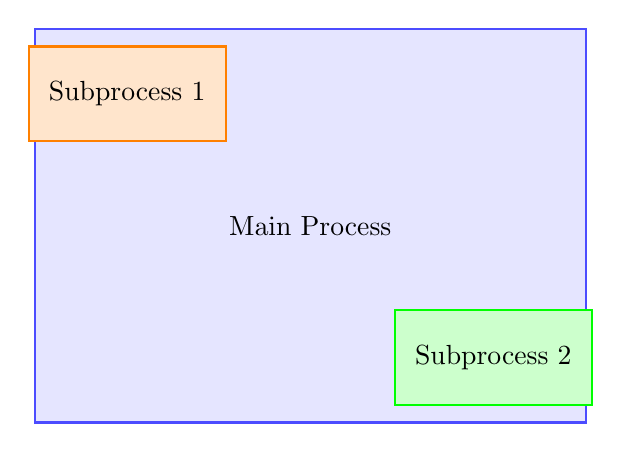
\begin{tikzpicture}[baseline=(current bounding box.center), node distance=1.5cm]
\node[draw=blue!70, thick, rectangle, minimum width=7cm, minimum height=5cm, align=center, fill=blue!10] (container) {Main Process};
\node[draw=orange, thick, rectangle, minimum width=2.5cm, minimum height=1.2cm, align=center, fill=orange!20, above left=of container.center] (sub1) {Subprocess 1};
\node[draw=green, thick, rectangle, minimum width=2.5cm, minimum height=1.2cm, align=center, fill=green!20, below right=of container.center] (sub2) {Subprocess 2};
\end{tikzpicture} \\[0.5em]
\textbf{Draw.io Translation:} Use a group rectangle for the main process, then place child rectangles inside to represent subprocesses. \\[0.5em]
\textbf{Key Parameters:} \texttt{minimum width/height, fill color, node positioning relative to container} \\
\hline
\end{longtable}

\newpage
\noindent
{\large \textbf{Content (fully worked out problems \& answers)}} \\

% Question 16: Parallel Merge
\begin{longtable}{|p{0.9\linewidth}|}
\hline
\textbf{(6)} How do you merge multiple parallel paths into a single node, like draw.io converging flows? \\[0.5em]
\textbf{Solution:} \\[0.5em]
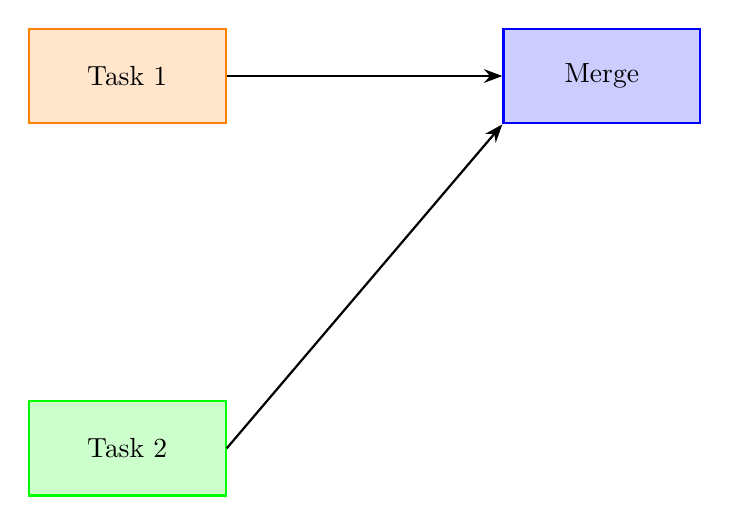
\begin{tikzpicture}[baseline=(current bounding box.center), node distance=3.5cm]
\node[draw=orange, thick, rectangle, minimum width=2.5cm, minimum height=1.2cm, align=center, fill=orange!20] (task1) {Task 1};
\node[draw=blue, thick, rectangle, minimum width=2.5cm, minimum height=1.2cm, align=center, fill=blue!20, right=of task1] (merge) {Merge};
\node[draw=green, thick, rectangle, minimum width=2.5cm, minimum height=1.2cm, align=center, fill=green!20, below=of task1] (task2) {Task 2};
\draw[-Stealth, thick] (task1.east) -- (merge.west);
\draw[-Stealth, thick] (task2.east) -- (merge.south west);
\end{tikzpicture} \\[0.5em]
\textbf{Draw.io Translation:} Connect two rectangles to a single target rectangle using straight or elbow connectors. Use consistent color coding. \\[0.5em]
\textbf{Key Parameters:} Connector direction and node alignment to create clean merge visualization \\
\hline
\end{longtable}

\newpage
\noindent
{\large \textbf{Content (fully worked out problems \& answers)}} \\

% Question 17: Conditional Loops
\begin{longtable}{|p{0.9\linewidth}|}
\hline
\textbf{(7)} How do you create a conditional loop with a back arrow for iteration, replicating draw.io loop connectors? \\[0.5em]
\textbf{Solution:} \\[0.5em]
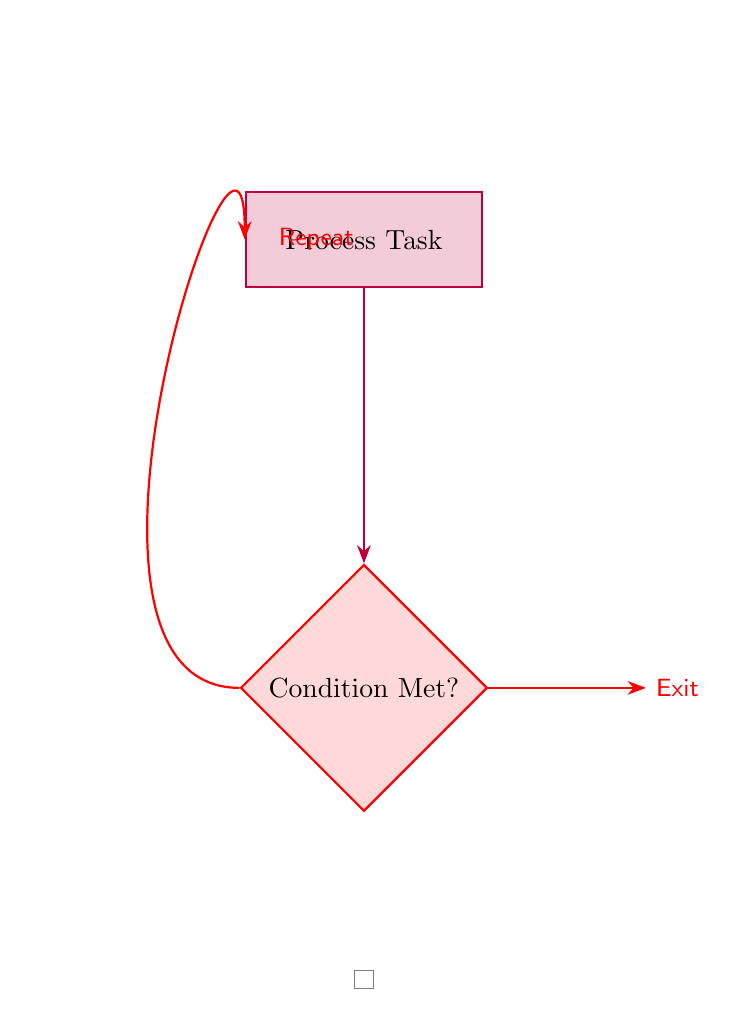
\begin{tikzpicture}[baseline=(current bounding box.center), node distance=3.5cm, auto]
\node[draw=purple, thick, rectangle, minimum width=3cm, minimum height=1.2cm, align=center, fill=purple!20] (process) {Process Task};
\node[draw=red, thick, diamond, minimum width=3cm, minimum height=1.5cm, align=center, fill=red!15, below=of process] (decision) {Condition Met?};
\node[draw=gray, minimum width=0pt, minimum height=0pt, below=2cm of decision] {}; % invisible node for spacing

\draw[-Stealth, thick, purple] (process) -- (decision.north);
\draw[-Stealth, thick, red, out=180, in=90, looseness=1.2] (decision.west) to (process.west) node[midway, left, font=\sffamily\small] {Repeat};
\draw[-Stealth, thick, red, out=0, in=90] (decision.east) -- ++(2,0) node[right, font=\sffamily\small] {Exit};
\end{tikzpicture} \\[0.5em]
\textbf{Draw.io Translation:} Use a rectangle for the process, diamond for the condition. Use a curved connector (orthogonal or bezier) looping back for "Repeat", straight arrow for "Exit". \\[0.5em]
\textbf{Key Parameters:} \texttt{out=180, in=90, looseness=1.2} controls smooth loop-back, labels positioned midway \\
\hline
\end{longtable}


\newpage
\noindent
{\large \textbf{Content (fully worked out problems \& answers)}} \\

% Question 18: Connector with Arrow Head Styles
\begin{longtable}{|p{0.9\linewidth}|}
\hline
\textbf{(8)} How do you change arrowhead styles on connectors to match draw.io options? \\[0.5em]
\textbf{Solution:} \\[0.5em]
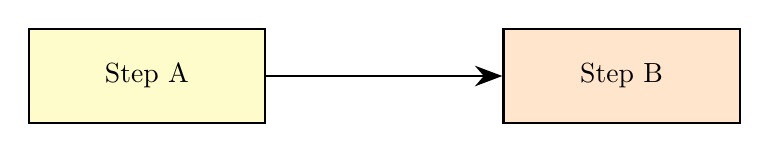
\begin{tikzpicture}[baseline=(current bounding box.center), node distance=3cm]
\node[draw=black, thick, rectangle, minimum width=3cm, minimum height=1.2cm, fill=yellow!20, align=center] (a) {Step A};
\node[draw=black, thick, rectangle, minimum width=3cm, minimum height=1.2cm, fill=orange!20, align=center, right=of a] (b) {Step B};
\draw[-{Stealth[scale=1.5]}, thick] (a) -- (b);
\end{tikzpicture} \\[0.5em]
\textbf{Draw.io Translation:} Select connector, change arrowhead style to classic, block, or diamond. Adjust size if needed. \\[0.5em]
\textbf{Key Parameters:} TikZ \texttt{-\{Stealth[scale=1.5]\}} controls arrowhead style \\
\hline
\end{longtable}

\newpage
\newpage
\noindent
{\large \textbf{Content (fully worked out problems \& answers)}} \\

% Question 19: Data Store Representation
\begin{longtable}{|p{0.9\linewidth}|}
\hline
\textbf{(9)} How do you represent a data store or database in TikZ similar to draw.io’s cylinder/data shapes? \\[0.5em]
\textbf{Solution:} \\[0.5em]
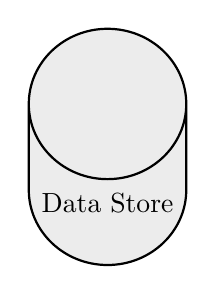
\begin{tikzpicture}[baseline=(current bounding box.center)]
\node[draw=black, thick, cylinder, shape border rotate=90, minimum width=2cm, minimum height=3cm, align=center, fill=gray!15] (data) {Data Store};
\end{tikzpicture} \\[0.5em]
\textbf{Draw.io Translation:} Use Cylinder shape from General or Database shapes. Set width=2cm, height=3cm, fill light gray, stroke black. \\[0.5em]
\textbf{Key Parameters:} \texttt{cylinder, shape border rotate=90, minimum width/height, fill=gray!15} \\
\hline
\end{longtable}

\newpage
\noindent
{\large \textbf{Content (fully worked out problems \& answers)}} \\

% Question 20: Event Start/End Circles
\begin{longtable}{|p{0.9\linewidth}|}
\hline
\textbf{(10)} How do you create start/end events with circles that correspond to draw.io’s BPMN events? \\[0.5em]
\textbf{Solution:} \\[0.5em]
\begin{tikzpicture}[baseline=(current bounding box.center)]
\node[draw=darkgreen, very thick, circle, minimum size=2cm, align=center, fill=green!10] (start) {Start};
\node[draw=red, very thick, circle, minimum size=2cm, align=center, fill=red!10, right=of start] (end) {End};
\draw[-Stealth, thick, darkgreen] (start) -- (end);
\end{tikzpicture} \\[0.5em]
\textbf{Draw.io Translation:} Use Circle shape for start and end events. Connect with arrow. Set fill colors and stroke thickness to match. \\[0.5em]
\textbf{Key Parameters:} \texttt{circle, minimum size, fill color, thick stroke} \\
\hline
\end{longtable}

\newpage
\noindent
{\large \textbf{Content (fully worked out problems \& answers)}} \\

% Question 21: Grouped Process Nodes
\begin{longtable}{|p{0.9\linewidth}|}
\hline
\textbf{(11)} How do you group multiple process nodes together to indicate a single module or stage, similar to draw.io groups? \\[0.5em]
\textbf{Solution:} \\[0.5em]
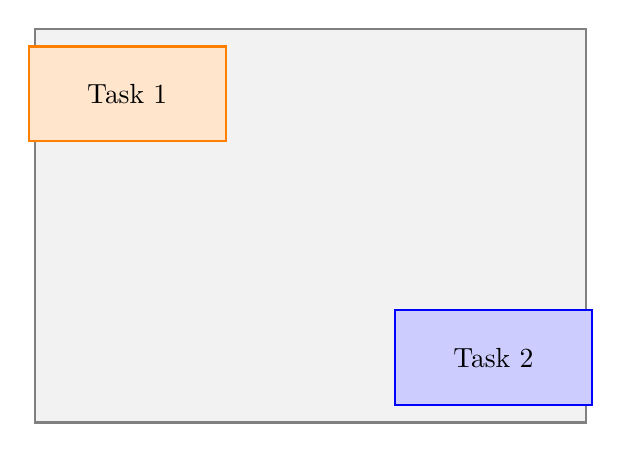
\begin{tikzpicture}[baseline=(current bounding box.center), node distance=1.5cm]
\node[draw=gray, thick, rectangle, minimum width=7cm, minimum height=5cm, fill=gray!10] (group) {};
\node[draw=orange, thick, rectangle, minimum width=2.5cm, minimum height=1.2cm, align=center, fill=orange!20, above left=of group.center] (p1) {Task 1};
\node[draw=blue, thick, rectangle, minimum width=2.5cm, minimum height=1.2cm, align=center, fill=blue!20, below right=of group.center] (p2) {Task 2};
\end{tikzpicture} \\[0.5em]
\textbf{Draw.io Translation:} Use a rectangle as a container, place child nodes inside, optionally add border/label to group. \\[0.5em]
\textbf{Key Parameters:} Node alignment relative to container, consistent color scheme \\
\hline
\end{longtable}

\newpage
\noindent
{\large \textbf{Content (fully worked out problems \& answers)}} \\

% Question 22: Swimlane with Multiple Lanes
\begin{longtable}{|p{0.9\linewidth}|}
\hline
\textbf{(12)} How do you construct a multi-lane swimlane diagram to show roles or departments, equivalent to draw.io swimlanes? \\[0.5em]
\textbf{Solution:} \\[0.5em]
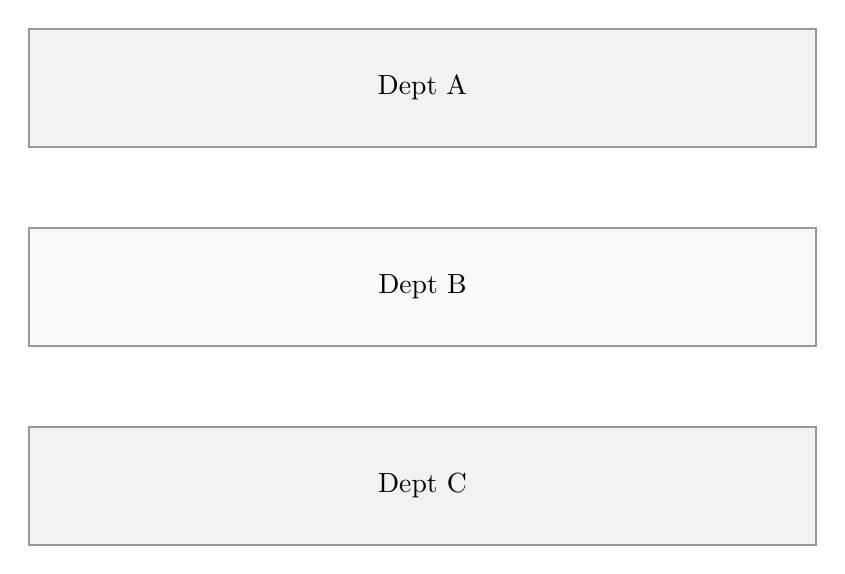
\begin{tikzpicture}[baseline=(current bounding box.center)]
\node[draw=gray!80, thick, rectangle, minimum width=10cm, minimum height=1.5cm, fill=gray!10] (lane1) {Dept A};
\node[draw=gray!80, thick, rectangle, minimum width=10cm, minimum height=1.5cm, fill=gray!05, below=of lane1] (lane2) {Dept B};
\node[draw=gray!80, thick, rectangle, minimum width=10cm, minimum height=1.5cm, fill=gray!10, below=of lane2] (lane3) {Dept C};
\end{tikzpicture} \\[0.5em]
\textbf{Draw.io Translation:} Use multiple horizontal swimlane shapes, alternating fill colors, label lanes for roles/departments. \\[0.5em]
\textbf{Key Parameters:} \texttt{rectangle, minimum width/height, fill alternating colors, label lanes} \\
\hline
\end{longtable}

\newpage
\noindent
{\large \textbf{Content (fully worked out problems \& answers)}} \\

% Question 23: Annotation Callout
\begin{longtable}{|p{0.9\linewidth}|}
\hline
\textbf{(13)} How do you add callout annotations or speech-bubble notes near a node, similar to draw.io callouts? \\[0.5em]
\textbf{Solution:} \\[0.5em]
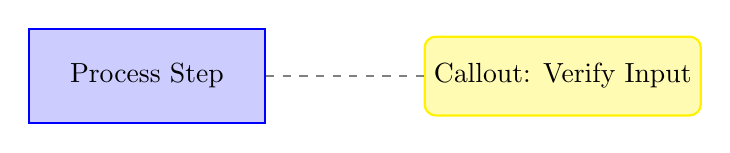
\begin{tikzpicture}[baseline=(current bounding box.center)]
\node[draw=blue, thick, rectangle, minimum width=3cm, minimum height=1.2cm, fill=blue!20] (task) {Process Step};
\node[draw=yellow, thick, rounded corners=4pt, minimum width=3cm, minimum height=1cm, align=left, fill=yellow!30, right=of task, xshift=1cm] (note) {Callout: Verify Input};
\draw[dashed, gray, -] (task.east) -- (note.west);
\end{tikzpicture} \\[0.5em]
\textbf{Draw.io Translation:} Use Callout or Rounded Rectangle for annotation, connect with dashed line to main node. \\[0.5em]
\textbf{Key Parameters:} \texttt{dashed, rounded corners, fill color, node positioning} \\
\hline
\end{longtable}

\newpage
\noindent
{\large \textbf{Content (fully worked out problems \& answers)}} \\

% Question 24: Connector with Multiple Waypoints
\begin{longtable}{|p{0.9\linewidth}|}
\hline
\textbf{(14)} How do you create connectors with multiple bends or waypoints, similar to draw.io polyline connectors? \\[0.5em]
\textbf{Solution:} \\[0.5em]
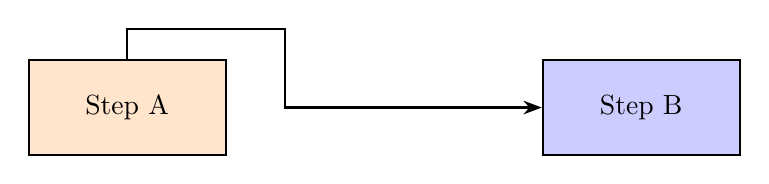
\begin{tikzpicture}[baseline=(current bounding box.center)]
\node[draw=black, thick, rectangle, minimum width=2.5cm, minimum height=1.2cm, fill=orange!20] (a) {Step A};
\node[draw=black, thick, rectangle, minimum width=2.5cm, minimum height=1.2cm, fill=blue!20, right=4cm of a] (b) {Step B};
\draw[-Stealth, thick] (a) |- ++(2,1) |- (b);
\end{tikzpicture} \\[0.5em]
\textbf{Draw.io Translation:} Use polyline connector, set multiple waypoints, optionally elbow style, arrowhead at target. \\[0.5em]
\textbf{Key Parameters:} \texttt{|-} for L-shapes in TikZ, equivalent to waypoints in draw.io \\
\hline
\end{longtable}

\newpage
\noindent
{\large \textbf{Content (fully worked out problems \& answers)}} \\

% Question 25: Advanced Themed Diagram
\begin{longtable}{|p{0.9\linewidth}|}
\hline
\textbf{(15)} How do you apply a professional color theme, shadows, and modern effects to match draw.io’s styled diagrams? \\[0.5em]
\textbf{Solution:} \\[0.5em]
\begin{tikzpicture}[
    baseline=(current bounding box.center),
    drop shadow/.style={
        general shadow={
            shadow xshift=2pt,
            shadow yshift=-2pt,
            draw=gray!50,
            fill=gray!20
        }
    }
]
\node[draw=blue!70, line width=2pt, rectangle, rounded corners=8pt, minimum width=3.5cm, minimum height=1.8cm, align=center, fill=blue!10, drop shadow, font=\sffamily\Large\bfseries, text=blue!80] (modern1) {Modern Step};
\node[draw=green!70, line width=2pt, rectangle, rounded corners=8pt, minimum width=3.5cm, minimum height=1.8cm, align=center, fill=green!15, drop shadow, font=\sffamily\Large\bfseries, text=green!70, right=of modern1] (modern2) {Enhanced Design};
\draw[-Stealth, line width=3pt, draw=purple!70, decoration={zigzag, segment length=4pt, amplitude=1pt}] (modern1) -- (modern2);
\end{tikzpicture} \\[0.5em]
\textbf{Draw.io Translation:} Use rounded rectangles with shadow effects, gradient fills, zigzag connectors, and consistent color theme. \\[0.5em]
\textbf{Key Parameters:} \texttt{rounded corners, line width, drop shadow, fill gradients, zigzag connector} \\
\hline
\end{longtable}
\newpage

\noindent
{\large \textbf{Checking for Understanding (questions \& answers)}} \\

\begin{longtable}{|p{0.9\linewidth}|}
\hline
\textbf{Core Principle 1: Interface Navigation} \\[0.5em]
\textbf{Three Main Panels:}
\begin{itemize}[leftmargin=1em]
\item \textbf{Left Panel:} Shape libraries (General, Flowchart, Business)
\item \textbf{Center Panel:} Canvas workspace
\item \textbf{Right Panel:} Format controls for selected objects
\end{itemize}
\textbf{Quick Start:} app.diagrams.net → Create New → Choose template \\
\\
\hline
\textbf{Core Principle 2: Precise Formatting} \\[0.5em]
\textbf{Dimension Control:} Right panel → Style → Position/Size \\
\textbf{Colors:} Fill/Line color → Custom → Hex codes \\
\textbf{Text:} Right panel → Text tab → Font properties \\
\textbf{Duplication:} Select → Ctrl+C → Ctrl+V → Arrange → Distribute horizontally \\
\\
\hline
\textbf{Core Principle 3: Connector Types} \\[0.5em]
\textbf{Connector Styles:}
\begin{itemize}[leftmargin=1em]
\item \textbf{Orthogonal:} Right-angle bends (flowcharts)
\item \textbf{Curved:} Smooth arcs (loop-backs)
\item \textbf{Straight:} Direct connections
\end{itemize}
\textbf{Labels:} Double-click connector → Add text → Position at connector midpoint \\
\\
\hline
\textbf{Core Principle 4: Layer Management} \\[0.5em]
\textbf{Access:} View → Layers (Ctrl+Shift+L) \\
\textbf{Organization:} Create named layers → Set Z-order → Lock completed layers \\
\textbf{Visibility:} Eye icon to show/hide layers \\
\textbf{Best Practice:} One active layer at a time, themed color schemes \\
\\
\hline
\textbf{Core Principle 5: Export \& Collaboration} \\[0.5em]
\textbf{Sharing:} File → Save As → Cloud storage → Set permissions \\
\textbf{Export Formats:}
\begin{itemize}[leftmargin=1em]
\item \textbf{PDF:} 300 DPI for print
\item \textbf{PNG:} 96 DPI for web, specify width
\end{itemize}
\textbf{Version Control:} Cloud auto-versioning + manual date stamps \\
\\
\hline
\end{longtable}
\newpage
\noindent
\section*{\underline{Activity 2}}
\begin{tabular}{|p{4.2cm}|p{9.8cm}|}
\hline
\textbf{Collaborative Learning Techniques} & Clusters \\
\hline
\textbf{Learning Strategy} & 3 Before Me \\
\hline
\textbf{Time} & 12:10---12:50 \\
\hline
\textbf{Materials} & A computer, OWLv2, textbook, canvas, anki, anki decks for download, ready to speak \\
\hline
\textbf{Lecture/Textbook/Old Plans/Slide References} & Anki, Canvas/Cengage, Chapter 1: Basic Concepts About Matter \\
\hline
\end{tabular}

\vspace{0.5cm}
\noindent
{\large \textbf{Instructions (please provide a \hl{DETAILED} activity breakdown below (and/or attached}} \\
\newpage
\begin{tabular}{|p{0.9\linewidth}|}
\hline
\begin{enumerate}
    \item \textbf{3 Before Me:} When a student asks a question during a session, have 3 students (or less depending on the number of students in the session) comment on a unique feature of that idea. The SI leader will mediate correct responses and help fill in gaps in understanding. This is a good strategy to model at the beginning of the semester and use throughout. This can help with redirecting questions and to encourage student-to-student interactions.
    \item \textbf{Activity 2}
    \item \textbf{Objective:} The students are going to be introduced to Canvas software by going through tasks which test their ability to navigate it and retrieve files as fast as they can.
    \item Each student will be asked to go on Canvas. If they are already familiar with Canvas, we will ask them to install Anki instead.
    \item Students will be encouraged to use AI tools (such as chat-based assistants) to gain general familiarity with Canvas, OWLv2, and the textbook interface. This can help them quickly understand how to navigate software and locate necessary materials.
    \item \textbf{Canvas}
    \begin{itemize}
        \item Once on Canvas, students will be asked to collapse all course fields and then open all fields to get an overview of the course layout.
        \item Canvas students will be asked to navigate to OWLv2 and ensure they have registered using their class code. Guidance on registration will be provided if needed.
        \item Canvas students will be instructed to open the course textbook through OWLv2 and explore the table of contents to locate chapters relevant to their assignments.
        \item Canvas students will also be instructed to explore the glossary for quick definitions of key terms and to look for practice problems associated with each chapter.
        \item Canvas students will locate the solutions section to check answers to practice problems after attempting them.
    \end{itemize}
    \item \textbf{Anki/Quizlet}
    \begin{itemize}
        \item Anki students will install their Anki distribution from the provided Linktree hub.
        \item Anki students will open Anki and complete an initial setup if prompted, including choosing language settings and syncing with an account if desired.
        \item Anki students will be guided to load pre-prepared decks either from shared files or by importing them from provided links.
        \item Anki students will learn to navigate the interface: reviewing cards, marking cards as correct or incorrect, and understanding spaced repetition scheduling.
        \item Anki students will be shown how to create their own cards, including using text, images, and basic formatting, to capture content from their course materials.
        \item Canvas students will return to OWLv2 and verify that they can access practice problem versions of their homework and understand how to submit assignments.
        \item Students in both groups will be encouraged to ask questions if they encounter difficulties and to use AI guidance as a tool for troubleshooting unfamiliar steps or software features.
    \end{itemize}
\end{enumerate} \\
\hline
\end{tabular}
\newpage
\noindent
{\large \textbf{Content (fully worked out problems \& answers)}} \\

\begin{tabular}{|p{0.9\linewidth}|}
\hline
\href{https://www.youtube.com/watch?v=Oq9EMmxF-DE}{Cengage OWLv2 Guide Video https://www.youtube.com/watch?v=Oq9EMmxF-DE}
\\ \hline
\includegraphics[width=0.9\textwidth]{pictures/CobbBrandonGraham_Stoker_Ch1_OWL_1_190825.png}
\\ \hline
\end{tabular}
\newpage
\noindent
{\large \textbf{Content (fully worked out problems \& answers)}} \\

\begin{tabular}{|p{0.9\linewidth}|}
\hline
\includegraphics[width=0.9\textwidth]{pictures/CobbBrandonGraham_Stoker_Ch1_OWL_2_190825.png}
\\ \hline
\end{tabular}
\newpage
\noindent
\section*{\underline{Closer}}
\begin{tabular}{|p{4.2cm}|p{9.8cm}|}
\hline
\textbf{Collaborative Learning Techniques} & Summarization \\
\hline
\textbf{Learning Strategy} & Group survey \\
\hline
\textbf{Time} & 12:50---12:55 \\
\hline
\textbf{Materials} & Pens, Flashcards \\
\hline
\textbf{Lecture/Textbook/Old Plans/Slide References} & Chapter 1: Basic Concepts of Matter \\
\hline
\end{tabular}

\vspace{0.5cm}
\noindent

\noindent
{\large \textbf{Instructions (please provide a \hl{DETAILED} activity breakdown below (and/or attached}}

\begin{tabular}{|p{0.9\linewidth}|}
\hline
\begin{enumerate}[itemsep=0.3em]
    \item Students write down the most important thing they learned
    \item Collect responses to inform next session
\end{enumerate}
\\ \hline
\end{tabular}

\vspace{0.5cm}
\noindent
{\large \textbf{Content (fully worked out problems \& answers)}}

\begin{tabular}{|p{0.9\linewidth}|}
\hline
\begin{itemize}
    \item No new worked problems; reflective summary
\end{itemize}
\\ \hline
\end{tabular}

\vspace{0.5cm}
\noindent
{\large \textbf{Checking for Understanding (questions \& answers)}}

\begin{tabular}{|p{0.9\linewidth}|}
\hline
\begin{itemize}
    \item Review student summaries
    \item Look for misunderstanding or unclear topics
\end{itemize}
\\ \hline
\end{tabular}
\newpage
\section*{Plan Checklist}

\begin{tabular}{|p{0.9\linewidth}|}
\hline
\begin{itemize}
\item[$\Box$] Variety of Collaborative Learning Techniques and Learning Strategies
\item[$\Box$] Chapter/slide \# where information is coming from
\item[$\Box$] Included timestamps (and buffer time as needed)
\item[$\Box$] Details on how leader will break up students
\item[$\Box$] Checking for Understanding questions
\item[$\Box$] Fully worked out problems and examples for each activity
\item[$\Box$] Necessary links required for online implementation (if applicable)
\item[$\Box$] Source material correctly cited (if applicable)
\item[$\Box$] Plan is uploaded to Teams
\end{itemize}
\\ \hline
\end{tabular}
\newpage

\end{document}

{\large \textbf{Checking for Understanding (questions \& answers)}} \\

\begin{tabular}{|p{0.9\linewidth}|}
\hline
\vspace{0.2cm}
\textbf{Questions:}
Is light considered matter? Why or why not? \\[1em]
If you filter seawater, what happens to its classification as a mixture? \\[1em]
Why is water (H$_2$O) a compound and not an element? \\[1em]
Why is density considered a physical property instead of a chemical property? \\[1em]
When salt dissolves in water, why is this considered a physical change? \\
Which state of matter has a definite shape and a definite volume? \\
If you cut a block of aluminum in half, which properties stay the same and which change? \\
Why must the total mass of reactants equal the total mass of products in a closed system? \\
Which of Dalton’s postulates was revised after the discovery of isotopes? \\
Give an everyday example of a homogeneous mixture and a heterogeneous mixture. \\


\hline
\begin{flushleft}
    \textbf{Answers:}   % Center the content within the table
    \begin{enumerate}
        \item \textbf{CFU 1: Matter vs. Energy} \\
        \item No — light is electromagnetic radiation, not matter. Light is carried by photons (symbol $\gamma$), which have zero rest mass ($m_0 = 0$) yet carry energy ($E = h\nu$) and momentum ($p = h/\lambda$). Matter, by the usual definition, consists of particles that have rest mass and occupy space; photons do not, so they are classified as energy. \\[1em]
        \item \textbf{CFU 2: Pure Substance vs. Mixture} \\
        \begin{enumerate}
            \item Filtration removes heterogeneous suspended solids, but dissolved ions remain.  
            \item Dissolved species such as $Na^+$ and $Cl^-$ remain uniformly distributed.  
            \item Therefore, seawater remains a homogeneous mixture (solution) after filtration.  
        \end{enumerate} \\[1em]
        \item \textbf{CFU 3: Elements and Compounds} \\
        \begin{enumerate}
            \item Water contains two different elements (hydrogen and oxygen) in a fixed ratio.  
            \item An element consists of only one type of atom; a compound consists of two or more types chemically bonded.  
            \item Breaking water into $H_2$ and $O_2$ requires a chemical reaction: $$2\,H_2O \rightarrow 2\,H_2 + O_2.$$  
        \end{enumerate} \\[1em]
        \item \textbf{CFU 4: Physical vs. Chemical Properties} \\
        \begin{enumerate}
            \item Density is defined as $\rho = \frac{m}{V}$.  
            \item Measuring density does not alter the chemical composition.  
            \item It is an intensive property: independent of sample size.  
        \end{enumerate} \\[1em]
        \item \textbf{CFU 5: Physical vs. Chemical Changes} \\
        \begin{enumerate}
            \item Salt dissociates into ions: $$NaCl_{(s)} \rightarrow Na^+_{(aq)} + Cl^-_{(aq)}.$$  
            \item No new chemical species are formed; chemical identity of ions remains.  
            \item The process is reversible (e.g., evaporation reforms $NaCl_{(s)}$).  
        \end{enumerate} \\[1em]
        \item \textbf{CFU 6: States of Matter} \\
        \begin{enumerate}
            \item Solids have definite shape and definite volume.  
            \item Liquids have definite volume but indefinite shape.  
            \item Gases have neither definite shape nor definite volume.  
        \end{enumerate} \\[1em]
        \item \textbf{CFU 7: Intensive vs. Extensive Properties} \\
        \begin{enumerate}
            \item Extensive properties (depend on sample size) change: mass $m$, volume $V$.  
            \item Intensive properties (independent of size) remain: density $\rho$, color, melting point $T_m$.  
            \item For density: $$\rho = \frac{m}{V} = \frac{m/2}{V/2} = \rho.$$  
        \end{enumerate} \\[1em]
        \item \textbf{CFU 8: Conservation of Mass} \\
        \begin{enumerate}
            \item Atoms are rearranged but not created or destroyed.  
            \item Total mass is conserved: $$\sum m_{\text{reactants}} = \sum m_{\text{products}}.$$  
            \item Example: $$2\,H_2 + O_2 \rightarrow 2\,H_2O$$ rearranges the same atoms; mass is unchanged.  
        \end{enumerate} \\[1em]
        \item \textbf{CFU 9: Atomic Theory} \\ 
        \begin{enumerate}
            \item Dalton’s claim that “atoms of the same element are identical in mass” was revised.  
            \item Isotopes ($^{12}C$, $^{14}C$) show atoms of the same element can differ in mass.  
            \item Chemical properties are similar; atomic masses can vary.  
        \end{enumerate} \\[1em]
        \item \textbf{CFU 10: Classification of Matter} \\
        \begin{enumerate}
            \item Homogeneous mixture: $NaCl_{(aq)}$, air — composition is uniform.  
            \item Heterogeneous mixture: salad, sand + water — composition varies visibly.  
        \end{enumerate} \\[1em]
    \end{enumerate}
\end{flushleft}
\\ \hline
\end{tabular}
write out a full latex problem(s) with solutions for a variety of real chemical equations with an identification of cations and anions, balancing the equation, types of reactions, endothermic and exothermic spontaneous non spontaneous equilibrium rate of reaction ice tables etc